%----------------------------------------------------------------------------
%Type of document
\documentclass{beamer}

%----------------------------------------------------------------------------
%Packages
\usepackage{amsmath}
\usepackage{hyperref}

%----------------------------------------------------------------------------
%Local adjustments of settings and definitions
\setcounter{MaxMatrixCols}{10}
\setbeamertemplate{caption}[numbered]
\definecolor{links}{HTML}{2A1B81}
\hypersetup{colorlinks,linkcolor=,urlcolor=links}

%----------------------------------------------------------------------------
%Beamer theme (Madrid and Frankfurt are good options)
\usetheme{Madrid}

%----------------------------------------------------------------------------
%Start document
\begin{document}

%----------------------------------------------------------------------------
%Front matter
\title[Introduction]{Introduction to Macroeconomics}
\author[Bidder]{Rhys Bidder}
\institute[FRBSF]{Federal Reserve Bank of San Francisco}
\date{Michaelmas Term 2019}
\maketitle

%----------------------------------------------------------------------------
%Main body

\begin{frame}{Disclaimer}

The views expressed in this presentation, and all errors and omissions, should be regarded as those solely of the authors, and are not necessarily those of the Federal Reserve Bank of San Francisco, the Federal Reserve Board of Governors or the Federal Reserve System.

\end{frame}


%----------------------------------------------------------------------------
\section{DSGE Models}
%----------------------------------------------------------------------------

\begin{frame}

\begin{center}
{\LARGE DSGE Models}
\end{center}

\end{frame}

%%%%%%%%%%%%%%%%%%%%%%%%%%%%%%%%%%%%%%%%%%%%%%%%%%%%%%%%%%%%%%%%%%%%%%%%%%%%%
%%%%%%%%%%%%%%%%%%%%%%%%%%%%%%%%%%%%%%%%%%%%%%%%%%%%%%%%%%%%%%%%%%%%%%%%%%%%%

\begin{frame}{Macroeconomics is Dynamic}

\begin{figure}
\centering
\label{fig:expectations}
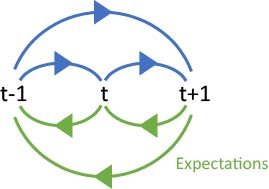
\includegraphics[width=0.3\textwidth]{Figures/ge_timing_expectations.JPG}
\end{figure}

Economic models are dynamic
\begin{itemize}
\item	They connect `yesterday' ($t-1$), `today' ($t$) and `tomorrow' ($t+1$)
\item	But so do other models (e.g. weather forecasting, bridge safety, \ldots)
\item	We share many tools with engineers, physicists\ldots	
\end{itemize}

Expectations are what make economics `special'
\begin{itemize}
\item	Our models (our world) are explicitly forward looking
\item	People make decisions with beliefs about the future in mind
\item	Aside: IoT, AI and machine learning?
\end{itemize}

\end{frame}

%%%%%%%%%%%%%%%%%%%%%%%%%%%%%%%%%%%%%%%%%%%%%%%%%%%%%%%%%%%%%%%%%%%%%%%%%%%%%
%%%%%%%%%%%%%%%%%%%%%%%%%%%%%%%%%%%%%%%%%%%%%%%%%%%%%%%%%%%%%%%%%%%%%%%%%%%%%

\begin{frame}{Macroeconomics is Stochastic}

Decision-makers must take randomness into account
\begin{itemize}
\item	Economists use the word `stochastic' to mean `randomness'
\end{itemize}
\vspace{2mm}	
We often don't know what's going to happen
\begin{itemize}
\item	We may not even know what has happened or is happening (filtering)
\end{itemize}
\vspace{2mm}
\textbf{Risk:} Even if we know how the world works there is still randomness
\begin{itemize}
\item	Playing a \textit{known} card game (don't know what's coming next but know the odds)
\end{itemize}
\vspace{2mm}
\textbf{Uncertainty:} There may also be `unknown unknowns' - \href{https://en.wikipedia.org/wiki/There_are_known_knowns}{Rumsfeld (2002)}
\begin{itemize}
\item	Like playing an \textit{unknown} card game (don't know what's coming next \textit{and} don't know the odds)
\end{itemize}

\end{frame}

%%%%%%%%%%%%%%%%%%%%%%%%%%%%%%%%%%%%%%%%%%%%%%%%%%%%%%%%%%%%%%%%%%%%%%%%%%%%%
%%%%%%%%%%%%%%%%%%%%%%%%%%%%%%%%%%%%%%%%%%%%%%%%%%%%%%%%%%%%%%%%%%%%%%%%%%%%%

\begin{frame}{Macroeconomics is Stochastic}

\begin{figure}
\centering
\label{fig:impulse_prop_fluct}
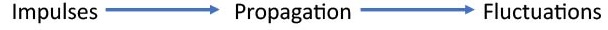
\includegraphics[width=0.5\textwidth]{Figures/impulse_prop_fluct.JPG}
\end{figure}

\textbf{Impulses:} Unexpected `structural shocks' to\ldots
	\begin{itemize}
	\item	Technology (ability to combine/reallocate resources effectively\ldots)
	\item	Monetary/fiscal policy (deviation from `standard' procedure, wars,\ldots)
	\item	Oil price, Forex and terms of trade (esp. for `small economies')
%	\item	`News' about future (forward guidance,\ldots)
	\end{itemize}
\vspace{1.5mm}
\textbf{Propagation:} How the shocks work their way through the system
	\begin{itemize}
	\item	Decisions by households and firms
	\item	Depends on preferences, technology, market structure, beliefs,\ldots
	\item	\textit{Modern} macro: explicitly microfounded and tightly parameterized
	\end{itemize}
\vspace{1.5mm}
\textbf{Fluctuations:} Due to shock propagation from current/previous periods
	\begin{itemize}
	\item	Equilibrium of a model $\Rightarrow$ probability distribution over `sequences'
	\item	Shocks and their propagation together define this distribution
	\end{itemize}

\end{frame}

%%%%%%%%%%%%%%%%%%%%%%%%%%%%%%%%%%%%%%%%%%%%%%%%%%%%%%%%%%%%%%%%%%%%%%%%%%%%%
%%%%%%%%%%%%%%%%%%%%%%%%%%%%%%%%%%%%%%%%%%%%%%%%%%%%%%%%%%%%%%%%%%%%%%%%%%%%%

\begin{frame}{Macroeconomics is General Equilibrium}

\begin{figure}
\centering
\label{fig:ge_feedback}
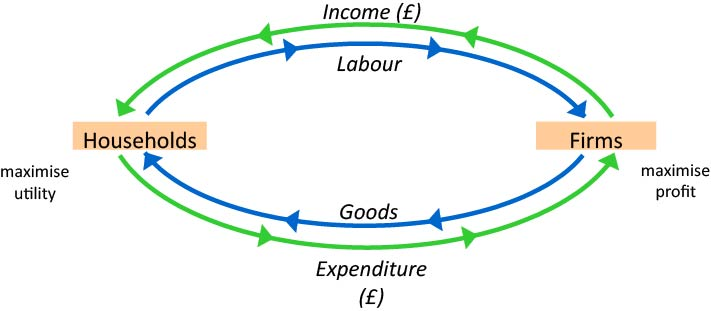
\includegraphics[width=0.3\textwidth]{Figures/ge_feedback.JPG}
\end{figure}
Markets are interconnected
	\begin{itemize}
	\item	We allow spillovers and connections between markets
	\item	Contrast with partial equilibrium (micro 101)
	\item	Typically variables are `simultaneously co-determined' in G.E.
	\end{itemize}
Simultaneity $\Rightarrow$ difficult to talk about causal relationships
	\begin{itemize}
	\item	Income depends on hours worked, depends on hiring, depends on scale of production, depends on demand, depends on income\ldots
	\end{itemize}
Interdependence of \textbf{individually optimal} decisions by multiple agents and \textbf{consistency} requirements in the aggregate
	\begin{itemize}
	\item	$\Rightarrow$ Set of simultaneous equations
	\end{itemize}

\end{frame}

%%%%%%%%%%%%%%%%%%%%%%%%%%%%%%%%%%%%%%%%%%%%%%%%%%%%%%%%%%%%%%%%%%%%%%%%%%%%%
%%%%%%%%%%%%%%%%%%%%%%%%%%%%%%%%%%%%%%%%%%%%%%%%%%%%%%%%%%%%%%%%%%%%%%%%%%%%%

\begin{frame}{Macroeconomics is General Equilibrium}

What does it mean to `solve' an economic model?
\begin{itemize}
\item	Models involve a lot of `variables' (consumption, unemployment, output, wages,\ldots)
\item	Accounting and technological constraints imply relationships among these variables
\item	The assumption that people and firms are optimizing also implies relationships among these variables
\item	There is a core set of variables that are needed to describe `the current situation' (all the relevant info.)
\item	We call these variables \textbf{`the state'}
\item	\textbf{Solving a model $\Leftrightarrow$ finding functions that relate all the variables in the economy to the state}
\end{itemize}

\end{frame}

%%%%%%%%%%%%%%%%%%%%%%%%%%%%%%%%%%%%%%%%%%%%%%%%%%%%%%%%%%%%%%%%%%%%%%%%%%%%%
%%%%%%%%%%%%%%%%%%%%%%%%%%%%%%%%%%%%%%%%%%%%%%%%%%%%%%%%%%%%%%%%%%%%%%%%%%%%%

\begin{frame}{Macroeconomics is General Equilibrium}

Remember high school math, when you had to `solve' systems of equations for $x_{1}$ and $x_{2}$
\begin{eqnarray*}
\alpha_{1,1}x_{1} + \alpha_{2,1}x_{2}	= y_{1} + z_{1}	\\
\alpha_{2,1}x_{1} + \alpha_{2,2}x_{2}	= y_{2} + z_{2}
\end{eqnarray*}
where the \textit{solution} will be $x_{1}=f_{1}(\alpha,y,z)$ and $x_{2}=f_{2}(\alpha,y,z)$

\vspace{3mm}
DSGE models' optimality conditions (Factor price ratio=MRT for firms, say) and equilibrium requirements (resource constraints, market clearing, belief consistency) will also yield a system of equations
	\begin{itemize}
	\item	More complicated (dynamics and expectations `replace' $y$ and $z$), but similar intuition
	\item	Express endogenous variables as functions of the state
	\item	The exact form of those functions will depend on the model's structure and parameters
	\end{itemize}

\end{frame}

%%%%%%%%%%%%%%%%%%%%%%%%%%%%%%%%%%%%%%%%%%%%%%%%%%%%%%%%%%%%%%%%%%%%%%%%%%%%%
%%%%%%%%%%%%%%%%%%%%%%%%%%%%%%%%%%%%%%%%%%%%%%%%%%%%%%%%%%%%%%%%%%%%%%%%%%%%%

\begin{frame}{Macroeconomics is General Equilibrium}

In practice, questions in the press are frequently poorly posed
	\begin{itemize}
	\item	\textbf{Q:} What happens to employment if inflation drops?
	\item	\textbf{A:} It depends. Is inflation falling because of looser policy or because there's been an unexpected improvement in technology?
	\end{itemize}
\vspace{2mm}
`Employment' and `inflation' are \textbf{endogenous and co-determined}
	\begin{itemize}
	\item	They may both be fluctuating because of other factors - rather than one causing the other
	\item	Causality may work in both directions via response of different agents
	\end{itemize}
\vspace{2mm}	
In micro 101 (and in a lot of old skool macro) these issues are brushed aside
	\begin{itemize}
	\item	Modern macro $\Rightarrow$ shocks are the exogenous `causal' source of fluctuations
	\item	Transmission mechanism (in equilibrium) then determines how variables co-move
	\end{itemize}

\end{frame}

%%%%%%%%%%%%%%%%%%%%%%%%%%%%%%%%%%%%%%%%%%%%%%%%%%%%%%%%%%%%%%%%%%%%%%%%%%%%%
%%%%%%%%%%%%%%%%%%%%%%%%%%%%%%%%%%%%%%%%%%%%%%%%%%%%%%%%%%%%%%%%%%%%%%%%%%%%%

\begin{frame}{DSGE models}

\begin{center}
\LARGE \textcolor{red}{D\ldots S\ldots GE}
\end{center}

Multiple periods \textcolor{red}{(D)}
	\begin{itemize}
	\item Agents form dynamic plans taking future into account
	\end{itemize}
Random shocks continually hitting the economy \textcolor{red}{(S)}
	\begin{itemize}
	\item From monetary policy and other sources (e.g. technology)
	\end{itemize}
Optimization problems of individual agents \textcolor{red}{(GE)}
	\begin{itemize}
	\item Preferences/profit maximization with budget/technological constraints
	\end{itemize}
Feasibility of optimal behavior in the aggregate \textcolor{red}{(GE)}
	\begin{itemize}
	\item Aggregation of individuals' decisions respects resource constraints
	\end{itemize}
Consistency of beliefs with the induced path of the economy \textcolor{red}{(GE)}
	\begin{itemize}
	\item Typically impose Rational Expectations requirement
	\end{itemize}

\end{frame}

%----------------------------------------------------------------------------
\section{Stylized Facts}
%----------------------------------------------------------------------------

\begin{frame}

\begin{center}
{\LARGE Stylized Facts}
\end{center}

\end{frame}

%%%%%%%%%%%%%%%%%%%%%%%%%%%%%%%%%%%%%%%%%%%%%%%%%%%%%%%%%%%%%%%%%%%%%%%%%%%%%
%%%%%%%%%%%%%%%%%%%%%%%%%%%%%%%%%%%%%%%%%%%%%%%%%%%%%%%%%%%%%%%%%%%%%%%%%%%%%

\begin{frame}{Macroeconomic fluctuations}

Decomposing fluctuations
	\begin{itemize}
	\item Underlying trend / low-frequency movements (`growth' literature)
	\item Business cycle
	\item Measurement error
	\item Seasonality (rarely discussed - let the statisticians handle it)
	\item `Random' fluctuations (`unmodelable' - or stuff we've failed to model)
	\end{itemize}
\vspace{3mm}
Growth and fluctuations can be connected as high frequency decisions can influence low frequency phenomena
	\begin{itemize}
	\item	Consume/save/innovate $\rightarrow$ investment/technology $\rightarrow$ growth
	\item	We will focus mainly on `business cycle' fluctuations
	\end{itemize}

\end{frame}

%%%%%%%%%%%%%%%%%%%%%%%%%%%%%%%%%%%%%%%%%%%%%%%%%%%%%%%%%%%%%%%%%%%%%%%%%%%%%
%%%%%%%%%%%%%%%%%%%%%%%%%%%%%%%%%%%%%%%%%%%%%%%%%%%%%%%%%%%%%%%%%%%%%%%%%%%%%

\begin{frame}{Macroeconomic data}

\begin{figure}
\caption[GNP-PCE]{Log GNP and consumption}
\centering
\label{fig:gnp_pce}
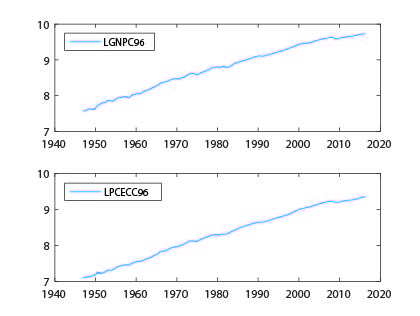
\includegraphics[width=0.45\textwidth]{Figures/gnp_pce.JPG}
\end{figure}

\begin{itemize}
\item	Note the fairly (until recently?) constant trend
\item	Long run co-movement between $Y$ and $C$
\item	Fluctuations around trend with a few big hits (recessions)
\end{itemize}

\end{frame}

%%%%%%%%%%%%%%%%%%%%%%%%%%%%%%%%%%%%%%%%%%%%%%%%%%%%%%%%%%%%%%%%%%%%%%%%%%%%%
%%%%%%%%%%%%%%%%%%%%%%%%%%%%%%%%%%%%%%%%%%%%%%%%%%%%%%%%%%%%%%%%%%%%%%%%%%%%%

\begin{frame}{Hodrick-Prescott Filter}

\href{https://en.wikipedia.org/wiki/Hodrick\%E2\%80\%93Prescott_filter}{Hodrick-Prescott filter} decomposes $y_{t}$ into trend, $\tau _{t}$, and cycle, $c_{t}$
\begin{equation*}
y_{t}=\tau _{t}+c_{t}
\end{equation*}

Trend should be `smooth' but track data closely in longer run
\begin{equation*}
\underset{\left\{ \tau _{t}\right\}_{t=1}^{T}}{\min}\left( \underbrace{\sum_{t=1}^{T}(y_{t}-\tau _{t})^{2}}_{Tracking}+\lambda \underbrace{\sum_{t=2}^{T-1}\left[ \left( \tau _{t+1}-\tau _{t}\right) -\left( \tau
_{t}-\tau _{t-1}\right) \right] ^{2}}_{Smoothness} \right)
\end{equation*}

$\lambda$ is weighting parameter
	\begin{itemize}
	\item $\lambda =0$ means $\tau _{t}=y_{t}$ and trend is data
	\item $\lambda \rightarrow \infty $ means $\Delta^{2}\tau_{t}=0$ and trend is linear
	\end{itemize}

\end{frame}

%%%%%%%%%%%%%%%%%%%%%%%%%%%%%%%%%%%%%%%%%%%%%%%%%%%%%%%%%%%%%%%%%%%%%%%%%%%%%%
%%%%%%%%%%%%%%%%%%%%%%%%%%%%%%%%%%%%%%%%%%%%%%%%%%%%%%%%%%%%%%%%%%%%%%%%%%%%%%

\begin{frame}{Hodrick-Prescott filter}

\begin{figure}
\caption[HP Trends]{Trend GNP using H-P filter}
\centering
\label{fig:gnp_different_hp}
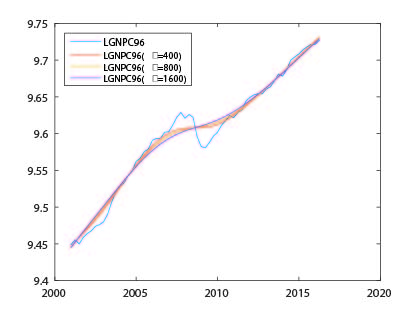
\includegraphics[width=0.35\textwidth]{Figures/gnp_different_hp.JPG}
\end{figure}

US GNP and H-P trends with different $\lambda$
\begin{itemize}
	\item	See \href{https://onlinelibrary.wiley.com/doi/abs/10.1002/jae.3950080302}{Harvey and Jaeger (1993)} on (in)appropriate use of HP filter
\end{itemize}
There are other ways of extracting trends
	\begin{itemize}
	\item	Linear (`draw a line through it')
	\item	Quadratic or cubic (`draw a bendy line through it')
	\item	Theoretical, rather than statistical (`use a model')
	\end{itemize}

\end{frame}

%%%%%%%%%%%%%%%%%%%%%%%%%%%%%%%%%%%%%%%%%%%%%%%%%%%%%%%%%%%%%%%%%%%%%%%%%%%%%%
%%%%%%%%%%%%%%%%%%%%%%%%%%%%%%%%%%%%%%%%%%%%%%%%%%%%%%%%%%%%%%%%%%%%%%%%%%%%%%

\begin{frame}{Hodrick-Prescott filter}

\begin{figure}
\caption[Power Transfer Function]{PTF of H-P filter with $\lambda =6400$ dots; $1600$ solid; $400$ dashes}
\centering
\label{fig:hp_ptf}
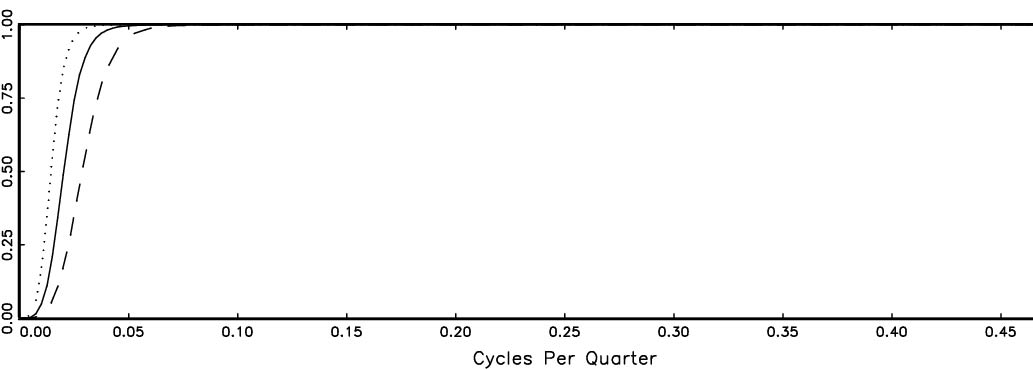
\includegraphics[width=0.40\textwidth]{Figures/hp_ptf.JPG}
\end{figure}

The \href{https://en.wikipedia.org/wiki/Filter_(signal_processing)\#The_transfer_function}{`power transfer function'} shows at what frequencies the \href{https://en.wikipedia.org/wiki/Filter_(signal_processing)}{filter} allows variation (e.g. $0.05$ cycles per quarter $\Rightarrow$ 5 years for a cycle)
	\begin{itemize}
	\item	Low frequencies: Few cycles per quarter (medium-long term trends)
	\item	High frequencies: Many cycles per quarter (business cycles and noise)
	\item	Variation in $y_{t}$ is a mix of \textit{all} frequencies - the filter lets through (\href{https://en.wikipedia.org/wiki/High-pass_filter\#/media/File:75_Hz_HPF_on_Smaart.jpg}{`passes'}) only a subset
	\end{itemize}
(Somewhat unconvincing) consensus that $\lambda =1600$ distinguishes `business cycle' and trend (quarterly data)
	\begin{itemize}
	\item	See also \href{https://www.mitpressjournals.org/doi/10.1162/003465399558454}{Baxter and King (2006)} \href{https://en.wikipedia.org/wiki/Band-pass_filter}{`band-pass'} filter
	\end{itemize}

\end{frame}

%%%%%%%%%%%%%%%%%%%%%%%%%%%%%%%%%%%%%%%%%%%%%%%%%%%%%%%%%%%%%%%%%%%%%%%%%%%%%%
%%%%%%%%%%%%%%%%%%%%%%%%%%%%%%%%%%%%%%%%%%%%%%%%%%%%%%%%%%%%%%%%%%%%%%%%%%%%%%

\begin{frame}{Long run properties of macro data}

\begin{figure}
\caption[HP Trend Growth Rate]{GNP and Trend Growth Rate ($\lambda=1600$)}
\centering
\label{fig:gnp_hp_trend}
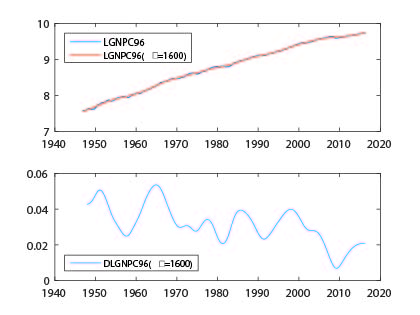
\includegraphics[width=0.40\textwidth]{Figures/gnp_hp_trend.JPG}
\end{figure}

Trend US growth `traditionally' thought of as $\approx 2.5-3.0\%$
	\begin{itemize}
	\item	GNP follows `straight line' in logs
	\end{itemize}
Note: Current debate about secular stagnation etc.
	\begin{itemize}
	\item	In U.S. labor force growth slowing and effects of `internet' subsiding
	\item	See \href{https://www.frbsf.org/economic-research/publications/economic-letter/2019/june/is-slow-still-new-normal-for-GDP-growth/}{Fernald and Li (2019)}
	\end{itemize}

\end{frame}

%%%%%%%%%%%%%%%%%%%%%%%%%%%%%%%%%%%%%%%%%%%%%%%%%%%%%%%%%%%%%%%%%%%%%%%%%%%%%%
%%%%%%%%%%%%%%%%%%%%%%%%%%%%%%%%%%%%%%%%%%%%%%%%%%%%%%%%%%%%%%%%%%%%%%%%%%%%%%

\begin{frame}{Long run properties of macro data}

\begin{figure}
\caption[Labor share and Great ratios]{Labor share and `Great Ratios'}
\centering
\label{fig:shares_ratios}
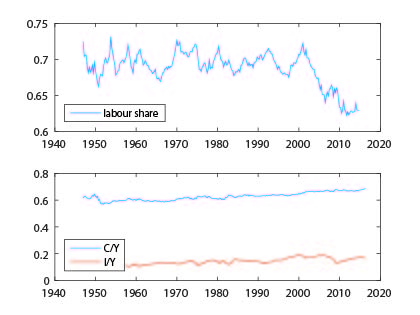
\includegraphics[width=0.30\textwidth]{Figures/shares_ratios.JPG}
\end{figure}

Fraction of output that goes to labor approximately constant
	\begin{itemize}
	\item	Or is it? \href{https://blogs.imf.org/2017/04/12/drivers-of-declining-labor-share-of-income/}{Big debate currently about declining ratio.}
	\item	Change in bargaining power, skills biased technical change, declining competition, \href{https://www.nber.org/papers/w19136.pdf}{cheaper investment goods}, \href{https://www.brookings.edu/bpea-articles/the-decline-of-the-u-s-labor-share/}{off-shoring}?
	\end{itemize}
`Great Ratios' (consumption and investment shares) $\approx$ constant
	\begin{itemize}
	\item	Maybe minor trend but these seem to be holding steady
	\end{itemize}

\end{frame}

%%%%%%%%%%%%%%%%%%%%%%%%%%%%%%%%%%%%%%%%%%%%%%%%%%%%%%%%%%%%%%%%%%%%%%%%%%%%%%
%%%%%%%%%%%%%%%%%%%%%%%%%%%%%%%%%%%%%%%%%%%%%%%%%%%%%%%%%%%%%%%%%%%%%%%%%%%%%%

\begin{frame}{Kaldor (1957) facts}

Kaldor's (1957) stylized facts have held up fairly well (subject to above caveats):
	\begin{enumerate}
	\item Output per worker grows at a roughly constant rate
	\item Capital per worker grows over time
	\item Capital/output ratio is roughly constant
	\item Rate of return to capital is constant
	\item Shares of capital and labor in net income are nearly constant
	\item Real wage grows over time
	\item Ratios of consumption and investment to GDP are constant
	\end{enumerate}

\end{frame}

%%%%%%%%%%%%%%%%%%%%%%%%%%%%%%%%%%%%%%%%%%%%%%%%%%%%%%%%%%%%%%%%%%%%%%%%%%%%%%
%%%%%%%%%%%%%%%%%%%%%%%%%%%%%%%%%%%%%%%%%%%%%%%%%%%%%%%%%%%%%%%%%%%%%%%%%%%%%%

\begin{frame}{Short run properties of macroeconomic data}

\begin{figure}
\caption[Detrended GNP and Consumption]{HP-Detrended GNP and Non-durable Consumption}
\centering
\label{fig:gnp_pce_hp_cycle}
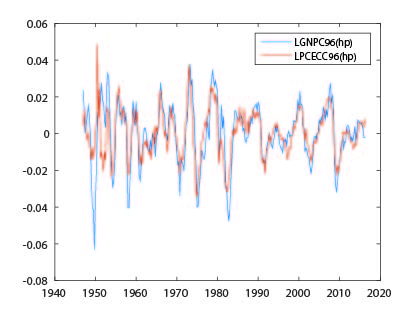
\includegraphics[width=0.55\textwidth]{Figures/gnp_pce_hp_cycle.JPG}
\end{figure}
\begin{itemize}
\item	Both series are `cyclical' components from HP filtering
\item	Strong positive correlation (consumption is `pro-cyclical')
\item	Consumption smoother than output. Why?
\end{itemize}

\end{frame}

%%%%%%%%%%%%%%%%%%%%%%%%%%%%%%%%%%%%%%%%%%%%%%%%%%%%%%%%%%%%%%%%%%%%%%%%%%%%%%
%%%%%%%%%%%%%%%%%%%%%%%%%%%%%%%%%%%%%%%%%%%%%%%%%%%%%%%%%%%%%%%%%%%%%%%%%%%%%%

\begin{frame}{Short run properties of macroeconomic data}

\begin{center}
\begin{table}
\label{tab:cross_corr}
\caption[Cross correlations]{Cyclical behavior of US economy $1954-1991$}
\begin{tabular}{|ccc|}
\hline
{\small Variable} & {\small Sd\%} & {\small Cross-correlation of output with:
} \\ \hline
\begin{tabular}{l}
\\ 
{\small GNP} \\ 
{\small CND} \\ 
{\small CD} \\ 
{\small I} \\ 
{\small H} \\ 
{\small Ave H} \\ 
{\small L} \\ 
{\small GNP/H} \\ 
{\small Ave W}
\end{tabular}
& 
\begin{tabular}{l}
\\ 
{\small 1.72} \\ 
{\small 0.86} \\ 
{\small 4.96} \\ 
{\small 8.24} \\ 
{\small 1.59} \\ 
{\small 0.63} \\ 
{\small 1.14} \\ 
{\small 0.90} \\ 
{\small 0.55}
\end{tabular}
& 
\begin{tabular}{ccccccc}
{\small t-3} & {\small t-2} & {\small t-1} & {\small t} & {\small t+1} & 
{\small t+2} & {\small t+3} \\ 
{\small 0.38} & {\small 0.63} & {\small 0.85} & {\small 1.00} & {\small 0.85}
& {\small 0.63} & {\small 0.38} \\ 
{\small 0.55} & {\small 0.68} & {\small 0.78} & {\small 0.77} & {\small 0.64}
& {\small 0.47} & {\small 0.27} \\ 
{\small 0.49} & {\small 0.65} & {\small 0.75} & {\small 0.78} & {\small 0.61}
& {\small 0.38} & {\small 0.11} \\ 
{\small 0.38} & {\small 0.59} & {\small 0.79} & {\small 0.91} & {\small 0.76}
& {\small 0.50} & {\small 0.22} \\ 
{\small 0.30} & {\small 0.53} & {\small 0.74} & {\small 0.86} & {\small 0.82}
& {\small 0.69} & {\small 0.52} \\ 
{\small 0.34} & {\small 0.48} & {\small 0.63} & {\small 0.62} & {\small 0.52}
& {\small 0.37} & {\small 0.23} \\ 
{\small 0.23} & {\small 0.46} & {\small 0.69} & {\small 0.85} & {\small 0.86}
& {\small 0.76} & {\small 0.59} \\ 
{\small 0.20} & {\small 0.30} & {\small 0.33} & {\small 0.41} & {\small 0.19}
& {\small 0.00} & {\small -0.18} \\ 
{\small 0.21} & {\small 0.14} & {\small 0.09} & {\small 0.03} & {\small -0.07
} & {\small -0.09} & {\small -0.09}
\end{tabular}
\\ \hline
\end{tabular}
\end{table}
\end{center}

\end{frame}

%%%%%%%%%%%%%%%%%%%%%%%%%%%%%%%%%%%%%%%%%%%%%%%%%%%%%%%%%%%%%%%%%%%%%%%%%%%%%%
%%%%%%%%%%%%%%%%%%%%%%%%%%%%%%%%%%%%%%%%%%%%%%%%%%%%%%%%%%%%%%%%%%%%%%%%%%%%%%

\begin{frame}{Stylized facts}

\begin{itemize}
\item 	Non-durable consumption less volatile than output (consumption smoothing)
\item 	Volatility of output and hours similar
\item 	Employment more volatile than average hours (extensive margin, offset by intensive)
\item 	Wages less volatile than productivity (smooth wages)
\item 	Productivity slightly pro-cyclical
\item 	Wage acyclical (despite employment volatility)
\end{itemize}

\end{frame}

%----------------------------------------------------------------------------
\section{Vector Autoregressions}
%----------------------------------------------------------------------------

\begin{frame}

\begin{center}
{\LARGE Vector Autoregressions}
\end{center}

\end{frame}

%%%%%%%%%%%%%%%%%%%%%%%%%%%%%%%%%%%%%%%%%%%%%%%%%%%%%%%%%%%%%%%%%%%%%%%%%%%%%%
%%%%%%%%%%%%%%%%%%%%%%%%%%%%%%%%%%%%%%%%%%%%%%%%%%%%%%%%%%%%%%%%%%%%%%%%%%%%%%

\begin{frame}{Vector autoregressions (VARs)}

Example: $p$-order VAR in two variables ($y_{t}$ and $x_{t}$)\ldots
\begin{eqnarray*}
y_{t} 	&=& a^{(1)}_{11}y_{t-1}+\ldots +a^{(p)}_{11}y_{t-p}+a^{(1)}_{12}x _{t-1}+\ldots+a^{(p)}_{12}x _{t-p}+u_{yt} \\
x _{t} 	&=&	a_{21}^{(1)}y_{t-1}+\ldots +a^{(p)}_{21}y_{t-p}+a^{(1)}_{22}x_{t-1}+\ldots +a^{(p)}_{22}x _{t-p}+u_{xt}
\end{eqnarray*}
\begin{itemize}
\item[]	where we imagine, say, $y_{t}$ being a measure of real activity and $x_{t}$ a measure of the stance of monetary policy (interest rate or money supply)
\end{itemize}
\vspace{1.5mm}
In matrix form\ldots
\begin{small}
\begin{equation*}
\begin{pmatrix}
y_{t} \\
x_{t}
\end{pmatrix}
= A(L)
\begin{pmatrix}
y_{t-1} \\
x_{t-1}
\end{pmatrix}
+
\begin{pmatrix}
u_{yt} \\
u_{xt}
\end{pmatrix}
\end{equation*}
\end{small}
\begin{itemize}
\item[]	where A(L) is a $p$-order matrix polynomial in the \href{https://en.wikipedia.org/wiki/Lag_operator}{lag operator} and $u_{it}$ is an innovation (`forecast error') to variable $i$.
\end{itemize}

\end{frame}

%%%%%%%%%%%%%%%%%%%%%%%%%%%%%%%%%%%%%%%%%%%%%%%%%%%%%%%%%%%%%%%%%%%%%%%%%%%%%%
%%%%%%%%%%%%%%%%%%%%%%%%%%%%%%%%%%%%%%%%%%%%%%%%%%%%%%%%%%%%%%%%%%%%%%%%%%%%%%

\begin{frame}{Vector Autoregressions}

Consider the special case of a VAR(1) ($p=1$)
\begin{equation*}
\begin{pmatrix}
y_{t} \\
x_{t}
\end{pmatrix}
=
\begin{pmatrix}
a_{11} 	& a_{12} \\
a_{21}	& a_{22}
\end{pmatrix}
\begin{pmatrix}
y_{t-1} \\
x_{t-1}
\end{pmatrix}
+
\begin{pmatrix}
u_{yt} \\
u_{xt}
\end{pmatrix}
\end{equation*}

Thus we have
\begin{eqnarray*}
y_{t} &=& a_{11} y_{t-1} + a_{12}x_{t-1} + u_{yt}	\\
x_{t} &=& a_{21} y_{t-1} + a_{22}x_{t-1} + u_{xt}
\end{eqnarray*}

Let us now consider the `forecast errors', $u_{yt}$ and $u_{xt}$\ldots

\end{frame}

%%%%%%%%%%%%%%%%%%%%%%%%%%%%%%%%%%%%%%%%%%%%%%%%%%%%%%%%%%%%%%%%%%%%%%%%%%%%%%
%%%%%%%%%%%%%%%%%%%%%%%%%%%%%%%%%%%%%%%%%%%%%%%%%%%%%%%%%%%%%%%%%%%%%%%%%%%%%%

\begin{frame}{Vector Autoregressions}

$x_{t}$ may not be what was expected at $t-1$ because 
\begin{itemize}
\item	the policymaker responded to surprises elsewhere in the economy in $t$
\item	the policymaker did something unexpected in a way unrelated to the broader economy (e.g. unexpected change in the voting patterns of a policy committee after new appointments)
\end{itemize}

\vspace{2mm}
We are interested in the effect of a \emph{policy surprise} (i.e. originating with the policymaker) rather than a surprise to the policy instrument, \emph{per se}
\begin{itemize}
\item	\textbf{But} without further assumptions $u_{xt}$ could be a combination of the desired `policy shock' and an `output shock' (such as a random loss in confidence by consumers, say)
\end{itemize}

\end{frame}

%%%%%%%%%%%%%%%%%%%%%%%%%%%%%%%%%%%%%%%%%%%%%%%%%%%%%%%%%%%%%%%%%%%%%%%%%%%%%%
%%%%%%%%%%%%%%%%%%%%%%%%%%%%%%%%%%%%%%%%%%%%%%%%%%%%%%%%%%%%%%%%%%%%%%%%%%%%%%

\begin{frame}{Vector Autoregressions}

$x_{t}$ may not be what was expected at $t-1$ because 
\begin{itemize}
\item	the policymaker responded to surprises elsewhere in the economy in $t$
\item	\textcolor{red}{the policymaker did something unexpected in a way unrelated to the broader economy (e.g. unexpected change in the voting patterns of a policy committee after new appointments)}
\end{itemize}

\vspace{2mm}
We are interested in the effect of a \textcolor{red}{\emph{policy surprise}} (i.e. originating with the policymaker) rather than a surprise to the policy instrument, \emph{per se}
\begin{itemize}
\item	\textbf{But} without further assumptions $u_{xt}$ could be a combination of the desired `policy shock' and an `output shock' (such as a random loss in confidence by consumers, say)
\end{itemize}

\end{frame}

%%%%%%%%%%%%%%%%%%%%%%%%%%%%%%%%%%%%%%%%%%%%%%%%%%%%%%%%%%%%%%%%%%%%%%%%%%%%%%
%%%%%%%%%%%%%%%%%%%%%%%%%%%%%%%%%%%%%%%%%%%%%%%%%%%%%%%%%%%%%%%%%%%%%%%%%%%%%%

\begin{frame}{Vector Autoregressions}

We can think of the forecast errors as being a linear combination of `structural' shocks, $e_{yt}$ and $e_{xt}$ where the latter is the `policy shock'
\begin{equation*}
\begin{pmatrix}
u_{yt} \\
u_{xt}
\end{pmatrix}
=
\begin{pmatrix}
e_{yt}+\theta e_{xt} \\
\phi e_{yt} + e_{xt}
\end{pmatrix}
=
\begin{pmatrix}
1 	& \theta \\
\phi & 1
\end{pmatrix}
\begin{pmatrix}
e_{yt} \\
e_{xt}
\end{pmatrix}
\equiv
B
\begin{pmatrix}
e_{yt} \\
e_{xt}
\end{pmatrix}
\end{equation*}

\vspace{2mm}
Without assumptions on $B$ (i.e. on $\theta$ and $\phi$ in this example) we cannot `pull apart' the forecast errors ($u_{it}$) and separately \textbf{identify} the effect of the structural shocks ($e_{it}$)
\begin{itemize}
\item	Example 1: Assume $\phi=0$
	\begin{itemize}
	\item	Policy variable does not respond contemporaneously to `output shocks'
	\end{itemize}
\item	Example 2: Assume $\theta=0$
	\begin{itemize}
	\item	Policy only affects output with a lag
	\end{itemize}
\item	Identified VAR is commonly referred to as a structural vector autoregression (SVAR)
\end{itemize}

\end{frame}
	
%%%%%%%%%%%%%%%%%%%%%%%%%%%%%%%%%%%%%%%%%%%%%%%%%%%%%%%%%%%%%%%%%%%%%%%%%%%%%%
%%%%%%%%%%%%%%%%%%%%%%%%%%%%%%%%%%%%%%%%%%%%%%%%%%%%%%%%%%%%%%%%%%%%%%%%%%%%%%

\begin{frame}{Vector Autoregressions}

Many identification schemes have been proposed (see Christiano \emph{et al} (1999) and Ramey (2016))
	\begin{itemize}
	\item	Two examples above are a case of using different `Cholesky' orderings
	\item	Ordering not unique and results may depend on ordering
	\item	Should have a plausible story
	\item	Logic extends to multiple shocks but more difficult to imagine a complete ordering
	\end{itemize}
Some famous examples of identification based on ordering\ldots
\begin{itemize}
\item	Sims (1992)
\item	Christiano, Eichenbaum and Evans (2005) - only used one ordering assumption
\end{itemize}

\end{frame}

%%%%%%%%%%%%%%%%%%%%%%%%%%%%%%%%%%%%%%%%%%%%%%%%%%%%%%%%%%%%%%%%%%%%%%%%%%%%%%
%%%%%%%%%%%%%%%%%%%%%%%%%%%%%%%%%%%%%%%%%%%%%%%%%%%%%%%%%%%%%%%%%%%%%%%%%%%%%%

\begin{frame}{Sims (1992)}

Six variable VAR for UK $1965-1990$ with causal ordering
	\begin{enumerate}
	\item Short interest rate ($R$)
	\item Index of foreign exchange value of domestic currency
	\item Commodity price index
	\item Monetary aggregate
	\item Consumer price index
	\item Industrial production index
	\end{enumerate}

\vspace{2mm}
Innovations only affect variables (weakly) lower in causal ordering
	\begin{itemize}
	\item	Interest rate first $\Rightarrow$ Central Bank not contemporaneously reacting to economic news
	\end{itemize}

\end{frame}

%%%%%%%%%%%%%%%%%%%%%%%%%%%%%%%%%%%%%%%%%%%%%%%%%%%%%%%%%%%%%%%%%%%%%%%%%%%%%%
%%%%%%%%%%%%%%%%%%%%%%%%%%%%%%%%%%%%%%%%%%%%%%%%%%%%%%%%%%%%%%%%%%%%%%%%%%%%%%

\begin{frame}{Sims (1992)}

\begin{figure}
\caption[Sims (1992) VAR]{Sims (1992) VAR for U.K. Economy}
\centering
\label{fig:sims_uk}
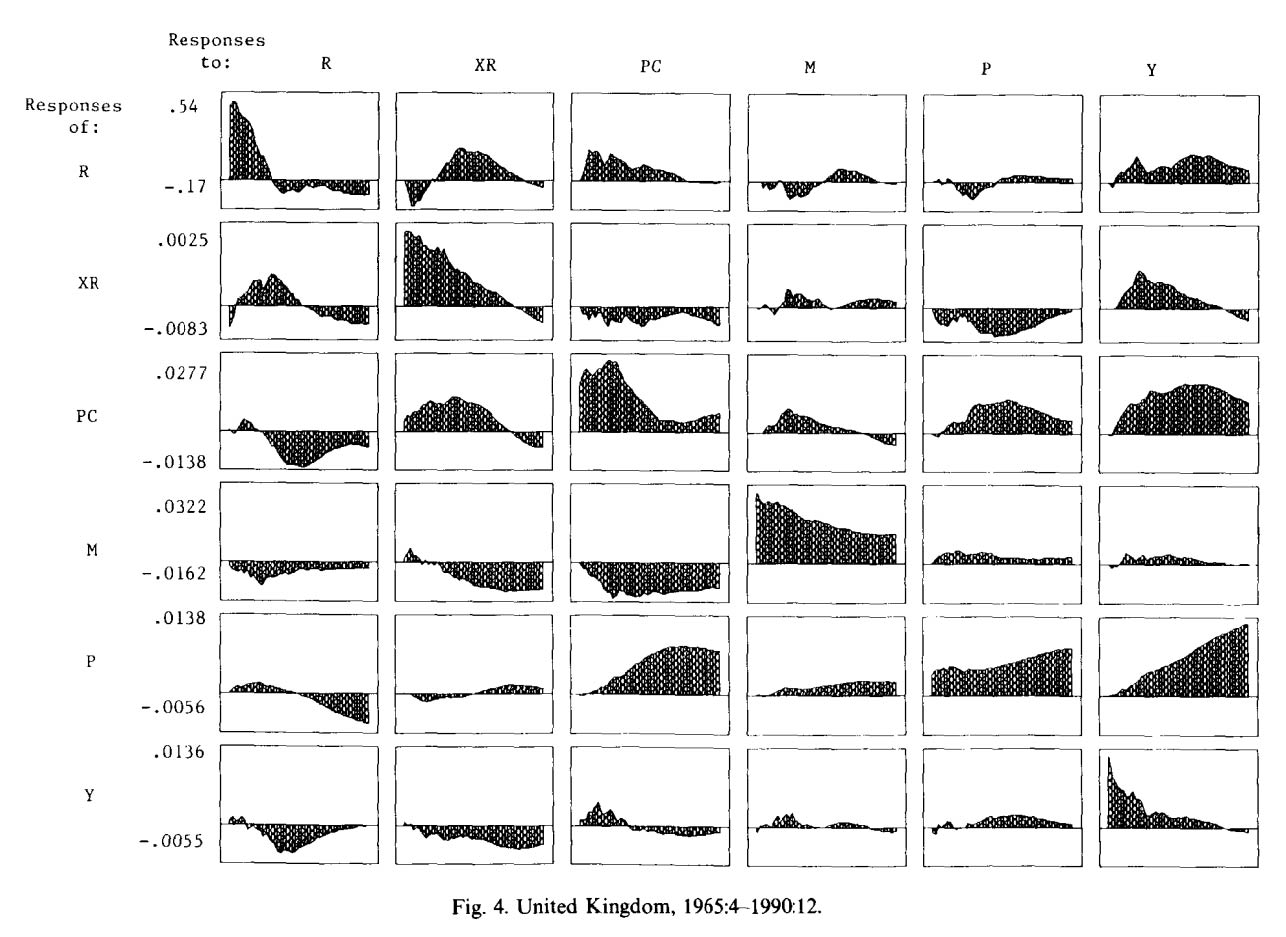
\includegraphics[width=0.65\textwidth]{Figures/sims_uk.JPG}
\end{figure}

\end{frame}

%%%%%%%%%%%%%%%%%%%%%%%%%%%%%%%%%%%%%%%%%%%%%%%%%%%%%%%%%%%%%%%%%%%%%%%%%%%%%%
%%%%%%%%%%%%%%%%%%%%%%%%%%%%%%%%%%%%%%%%%%%%%%%%%%%%%%%%%%%%%%%%%%%%%%%%%%%%%%

\begin{frame}{Christiano, Eichenbaum and Evans (2005)}

Nine variable VAR for US $1965-1995$ with causal ordering
	\begin{enumerate}
	\item 	Real GDP
	\item	Real consumption
	\item	GDP deflator
	\item	Real investment
	\item	Real wage
	\item	Labor productivity
	\item 	Interest rate
	\item 	Real profit
	\item	Growth rate of M2
	\end{enumerate}

Implications of position of $R$:
	\begin{itemize}	
	\item	$R$ Shocks only affect real profit and M2
	\item	$R$ Affected by all shocks except real profit and M2 shocks
	\end{itemize}

\end{frame}

%%%%%%%%%%%%%%%%%%%%%%%%%%%%%%%%%%%%%%%%%%%%%%%%%%%%%%%%%%%%%%%%%%%%%%%%%%%%%%
%%%%%%%%%%%%%%%%%%%%%%%%%%%%%%%%%%%%%%%%%%%%%%%%%%%%%%%%%%%%%%%%%%%%%%%%%%%%%%

\begin{frame}{Christiano, Eichenbaum and Evans (2005)}

Results suggest that after an expansionary monetary policy shock:
\begin{enumerate}
\item 	Output, consumption, and investment respond in a hump-shape, peaking after about one and a half years and returning to pre-shock levels after about three years
\item 	Inflation responds in a hump-shape, peaking after about two years
\item 	Interest rate falls for roughly one year
\item 	Real profits, real wages, and labor productivity rise
\item 	Growth rate of money rises immediately
\end{enumerate}

\end{frame}

%%%%%%%%%%%%%%%%%%%%%%%%%%%%%%%%%%%%%%%%%%%%%%%%%%%%%%%%%%%%%%%%%%%%%%%%%%%%%%
%%%%%%%%%%%%%%%%%%%%%%%%%%%%%%%%%%%%%%%%%%%%%%%%%%%%%%%%%%%%%%%%%%%%%%%%%%%%%%

\begin{frame}{Christiano, Eichenbaum and Evans (2005)}

\begin{figure}
\caption[CEE - Subset 1]{CEE (2005) - Impulse responses (I)}
\centering
\label{fig:cee_responses}
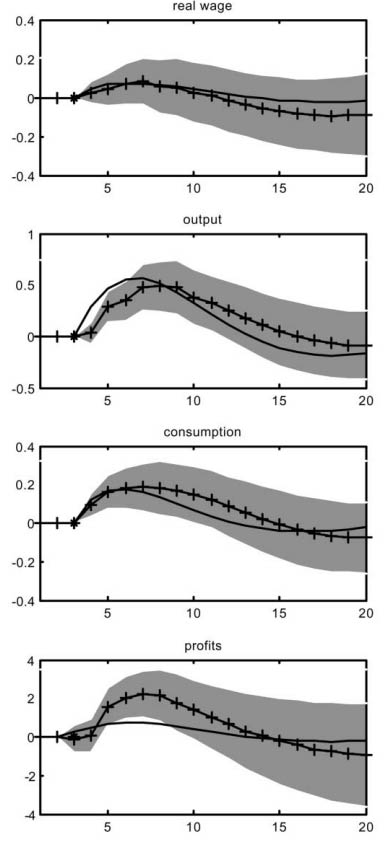
\includegraphics[width=0.25\textwidth]{Figures/cee_responses.JPG}
\end{figure}

\end{frame}

%%%%%%%%%%%%%%%%%%%%%%%%%%%%%%%%%%%%%%%%%%%%%%%%%%%%%%%%%%%%%%%%%%%%%%%%%%%%%%
%%%%%%%%%%%%%%%%%%%%%%%%%%%%%%%%%%%%%%%%%%%%%%%%%%%%%%%%%%%%%%%%%%%%%%%%%%%%%%

\begin{frame}{Christiano, Eichenbaum and Evans (2005)}

\begin{figure}
\caption[CEE - Subset 1]{CEE (2005) - Impulse responses (II)}
\centering
\label{fig:more_cee_responses}
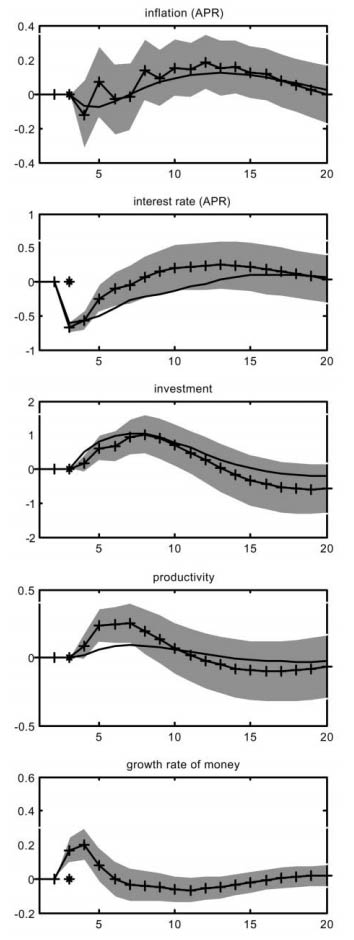
\includegraphics[width=0.20\textwidth]{Figures/more_cee_responses.JPG}
\end{figure}

\end{frame}

%%%%%%%%%%%%%%%%%%%%%%%%%%%%%%%%%%%%%%%%%%%%%%%%%%%%%%%%%%%%%%%%%%%%%%%%%%%%%%
%%%%%%%%%%%%%%%%%%%%%%%%%%%%%%%%%%%%%%%%%%%%%%%%%%%%%%%%%%%%%%%%%%%%%%%%%%%%%%

\begin{frame}{Problems with causal orderings}

Sims (1992) and CEE (2005) find prices initially $\uparrow $ after unexpected $R_{t} \uparrow$
	\begin{itemize}
	\item	Often referred to as the `price puzzle'
	\item 	Could be a cost channel effect (firm borrowing costs rise so they increase prices) but more likely faulty identification	
	\item	Thoughts on other possible explanations?
	\end{itemize}
\vspace{2mm}
Sign restriction VARs designed to rule out such anomalies
	\begin{itemize}
	\item	Impose restrictions not by ordering but by restricting which direction variables should move in following a shock
	\item	See Canova (2007), Canova and Paustian (2010), Uhlig (1998), Rubio-Ramirez (2018)
	\item	Though if the problem is incorrect set of variables (information for forecast) then might not help?
	\end{itemize}

\end{frame}

%%%%%%%%%%%%%%%%%%%%%%%%%%%%%%%%%%%%%%%%%%%%%%%%%%%%%%%%%%%%%%%%%%%%%%%%%%%%%%
%%%%%%%%%%%%%%%%%%%%%%%%%%%%%%%%%%%%%%%%%%%%%%%%%%%%%%%%%%%%%%%%%%%%%%%%%%%%%%

\begin{frame}{Sign restrictions}

\begin{figure}
\caption[Canov 2007]{Canova (2007) - Comparing responses to a monetary tightening based on Cholesky and Sign restrictions}
\centering
\label{fig:sign_vs_chol_irfs}
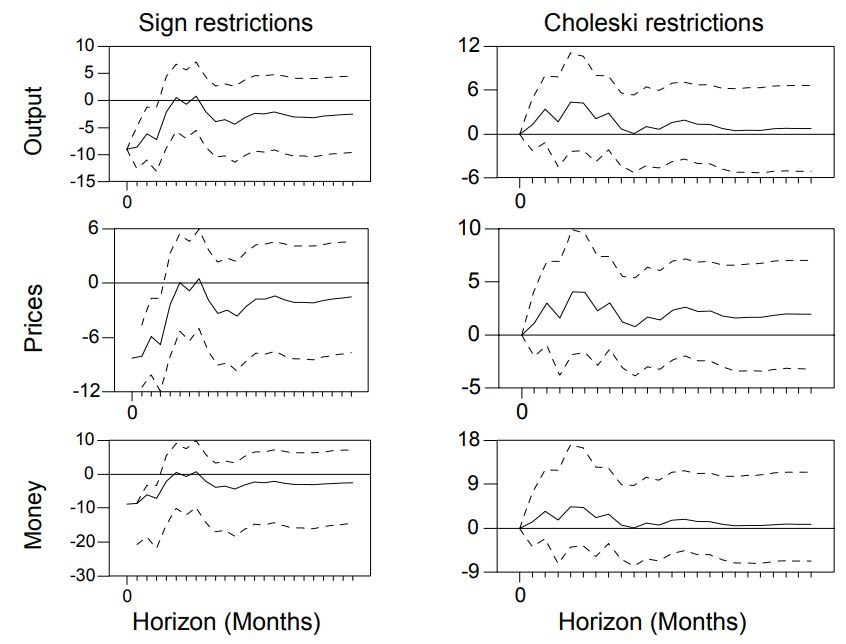
\includegraphics[width=0.60\textwidth]{Figures/sign_vs_chol_irfs.JPG}
\end{figure}

\end{frame}

%%%%%%%%%%%%%%%%%%%%%%%%%%%%%%%%%%%%%%%%%%%%%%%%%%%%%%%%%%%%%%%%%%%%%%%%%%%%%%
%%%%%%%%%%%%%%%%%%%%%%%%%%%%%%%%%%%%%%%%%%%%%%%%%%%%%%%%%%%%%%%%%%%%%%%%%%%%%%

\begin{frame}{Sign restrictions}

\begin{figure}
\caption[Canova and Paustian 2010]{Canova and Paustian (2010) - Sign restrictions}
\centering
\label{fig:sign_restrictions}
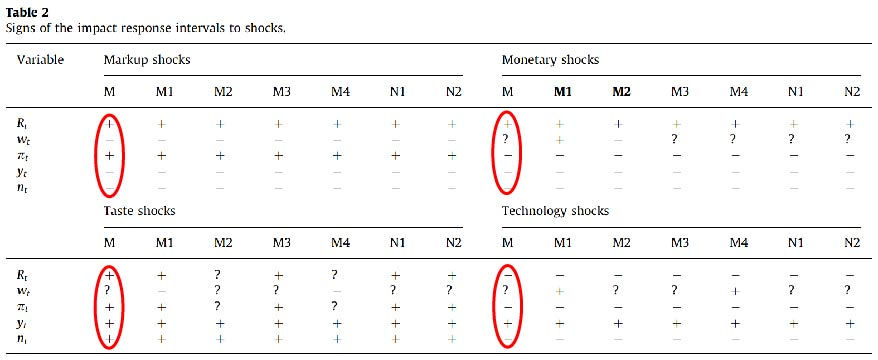
\includegraphics[width=1.0\textwidth]{Figures/sign_restrictions.JPG}
\end{figure}

\end{frame}

%%%%%%%%%%%%%%%%%%%%%%%%%%%%%%%%%%%%%%%%%%%%%%%%%%%%%%%%%%%%%%%%%%%%%%%%%%%%%%
%%%%%%%%%%%%%%%%%%%%%%%%%%%%%%%%%%%%%%%%%%%%%%%%%%%%%%%%%%%%%%%%%%%%%%%%%%%%%%

\begin{frame}{Identification using high frequency information}

\begin{itemize}
\item ECB monthly press conference January 15, 2009
\item Traders expect interest rate cut on February 5, 2009
\item Trichet announces no policy change expected next meeting
\item Traders revise up expectations
\end{itemize}

\end{frame}

%%%%%%%%%%%%%%%%%%%%%%%%%%%%%%%%%%%%%%%%%%%%%%%%%%%%%%%%%%%%%%%%%%%%%%%%%%%%%%
%%%%%%%%%%%%%%%%%%%%%%%%%%%%%%%%%%%%%%%%%%%%%%%%%%%%%%%%%%%%%%%%%%%%%%%%%%%%%%

\begin{frame}{Rosa (2008)}

\begin{figure}
\caption[Rosa (2008)]{Rosa (2008) - Mid-quote on 3-month Euribor future expiring in 03/09}
\centering
\label{fig:trichet_mkt_react}
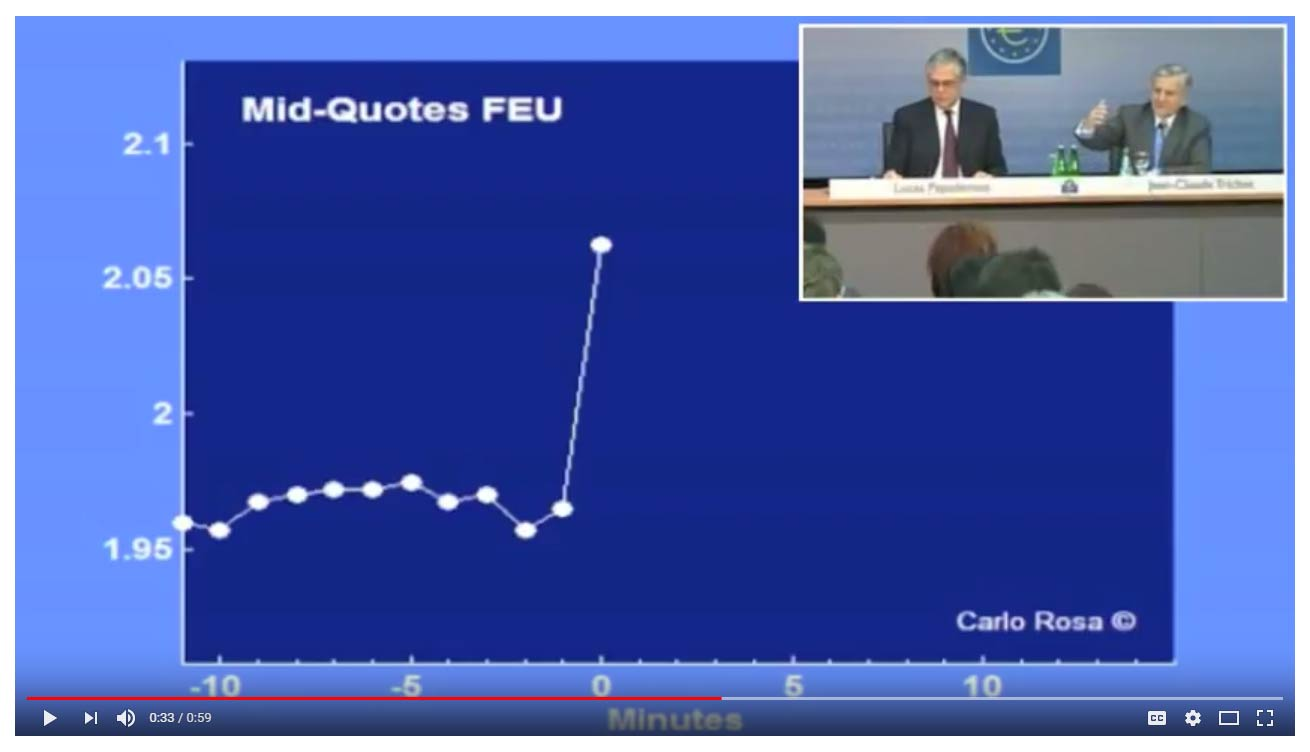
\includegraphics[width=0.45\textwidth]{Figures/trichet_mkt_react.JPG}
\end{figure}

Time zero when Trichet starts answering a journalist's question
\begin{itemize}
\item	Presumption is that nothing else `changes' during the short period from just before to just after $\Rightarrow$ Simply captures policy-surprise
\item	NOTE: Current debate about whether the CB is revealing info about the rest of the economy (as opposed to simply about monetary policy)
\end{itemize}

\end{frame}

%%%%%%%%%%%%%%%%%%%%%%%%%%%%%%%%%%%%%%%%%%%%%%%%%%%%%%%%%%%%%%%%%%%%%%%%%%%%%%%%
%%%%%%%%%%%%%%%%%%%%%%%%%%%%%%%%%%%%%%%%%%%%%%%%%%%%%%%%%%%%%%%%%%%%%%%%%%%%%%%%
%
%\begin{frame}{Kuttner (2001)}
%
%Spot-month futures rate on day $t$ of month $s$ interpreted as conditional expectation of the average funds rate in month $s$ plus term premium
%\begin{equation*}
%f_{s,t}^{0}=E_{t}\frac{1}{m}\sum\limits_{i\in s}r_{i}+\mu_{s,t}^{0}
%\end{equation*}
%
%Policy surprise measure computed from the 1-day change in the spot-month future rate
%\begin{equation*}
%\Delta \tilde{r}_{t}^{u}=\frac{m}{m-t}\left( f_{s,t}^{0}-f_{s,t-1}^{0}\right)
%\end{equation*}
%
%Surprise is proxied by change in futures rate
%\begin{itemize}
%\item	Leads to what is known as a `proxy VAR'
%\end{itemize}
%
%\end{frame}
%
%%%%%%%%%%%%%%%%%%%%%%%%%%%%%%%%%%%%%%%%%%%%%%%%%%%%%%%%%%%%%%%%%%%%%%%%%%%%%%%%
%%%%%%%%%%%%%%%%%%%%%%%%%%%%%%%%%%%%%%%%%%%%%%%%%%%%%%%%%%%%%%%%%%%%%%%%%%%%%%%%
%
%\begin{frame}{Proxy VAR}
%
%Correlated with both reduced form residuals but with only one structural innovation
%\begin{itemize}
%\item[] $E(e_{yt}z_{t})=\phi $
%\item[] $E(e_{xt}z_{t})=0$
%\end{itemize}
%\begin{equation*}
%\; \; \; \; \:E\left[ \left( 
%\begin{array}{c}
%u_{yt} \\ 
%u_{xt}
%\end{array}
%\right) z_{t}\right] =E\left[ \left( 
%\begin{array}{cc}
%\theta _{1} & \theta _{2} \\ 
%\theta _{3} & \theta _{4}
%\end{array}
%\right) \left( 
%\begin{array}{c}
%e_{yt} \\ 
%e_{xt}
%\end{array}
%\right) \left( \phi e_{yt}+\nu _{t}\right) \right] =\left( 
%\begin{array}{c}
%\theta _{1}\phi \\ 
%\theta _{3}\phi
%\end{array}
%\right)
%\end{equation*}
%
%\vspace{3mm}
%Thus, proxy VAR\ identified by restriction\ldots
%\begin{equation*}
%\frac{\theta _{1}}{\theta _{3}}=\frac{E(u_{yt}z_{t})}{E(u_{xt}z_{t})}
%\end{equation*}
%\begin{itemize}
%\item[] for known $E(u_{yt}z_{t})$ and $E(u_{xt}z_{t})$ (can be estimated from the reduced form VAR residuals and the constructed instrument, $z_{t}$)
%\end{itemize}
%
%\end{frame}

%%%%%%%%%%%%%%%%%%%%%%%%%%%%%%%%%%%%%%%%%%%%%%%%%%%%%%%%%%%%%%%%%%%%%%%%%%%%%%
%%%%%%%%%%%%%%%%%%%%%%%%%%%%%%%%%%%%%%%%%%%%%%%%%%%%%%%%%%%%%%%%%%%%%%%%%%%%%%

\begin{frame}{Vector Autoregressions}

\begin{quotation}
While researchers have disagreed on the best means of identifying policy shocks, there has been a surprising consensus on the general nature of the economic responses to monetary policy shocks. A variety of VARs estimated for a number of countries all indicate that, in response to a policy shocks, output follows a hump-shaped pattern in which the peak impact occurs several quarters after the initial shock.
\end{quotation}
\center - Walsh, 1998, p.31

\end{frame}

%%%%%%%%%%%%%%%%%%%%%%%%%%%%%%%%%%%%%%%%%%%%%%%%%%%%%%%%%%%%%%%%%%%%%%%%%%%%%%%
%%%%%%%%%%%%%%%%%%%%%%%%%%%%%%%%%%%%%%%%%%%%%%%%%%%%%%%%%%%%%%%%%%%%%%%%%%%%%%%
%
%\begin{frame}{Vector Autoregressions}
%
%VAR approach useful but not without flaws/critics\ldots
%\vspace{2mm}
%\begin{itemize}
%\item 	Monetary policy shocks are now likely rare/small (Ramey (2016))
%	\begin{itemize}
%	\item	Makes it more difficult to use \emph{policy} shocks to estimate impact of policy
%	\item	Can still estimate role of policy but need \emph{other} shocks \textbf{and} a model
%	\end{itemize}
%\vspace{1mm}
%\item	Changes in underlying parameters (Lucas critique and Rational Expectations)
%	\begin{itemize}
%	\item	Response to shocks depends on parameters describing policymakers' approach \textbf{and} all other parameters in the economy (e.g. regulation, preferences\ldots)
%	\item	If they change, previous estimates may become obsolete
%	\end{itemize}
%\vspace{1mm}	
%\item 	Responses may not be accurately recovered even from data generated by a model (Chari \emph{et al} (2008))
%	\begin{itemize}
%	\item	Can still use, but in a `moment matching' exercise \emph{involving a model}
%	\item	VARs on actual data and on data from model - minimize discrepancy
%	\end{itemize}
%\end{itemize}
%
%\end{frame}
%
%%%%%%%%%%%%%%%%%%%%%%%%%%%%%%%%%%%%%%%%%%%%%%%%%%%%%%%%%%%%%%%%%%%%%%%%%%%%%%%
%%%%%%%%%%%%%%%%%%%%%%%%%%%%%%%%%%%%%%%%%%%%%%%%%%%%%%%%%%%%%%%%%%%%%%%%%%%%%%%
%
%\begin{frame}{Vector Autoregressions}
%
%More problems with VAR analysis\ldots
%\vspace{2mm}
%\begin{itemize}
%\item	Unhelpful for welfare analysis
%	\begin{itemize}
%	\item	Knowing that policy affects activity is one thing\ldots
%	\item 	\ldots but knowing \emph{how it should try to affect it} is another
%	\item 	Agent's optimization problems must be explicit for micro-founded welfare analysis
%	\item 	VARs are silent on this
%	\end{itemize}
%\item	Story telling / incorporation of microeconomic evidence
%	\begin{itemize}
%	\item 	Policymakers like to understand/explain transmission mechanism
%	\item	Elements of models (such as, say, household risk aversion) can be pinned down by evidence from experiments/more granular research
%	\item	Not possible with VARs (or very difficult)
%	\end{itemize}
%\end{itemize}
%
%\vspace{2mm}
%A lot of these `problems' can be addressed by using a model\ldots
%
%\end{frame}



%----------------------------------------------------------------------------
\section{Some math(s)}
%----------------------------------------------------------------------------

\begin{frame}

\begin{center}
{\LARGE Appendix: Some math(s)}
\end{center}

\end{frame}

%----------------------------------------------------------------------------

%----------------------------------------------------------------------------

\begin{frame}{Unofficial maths `requirements'}

Most of the maths we use will entail\ldots
\begin{itemize}
\item	Basic algebra
	\begin{itemize}
	\item	$C_{t}$ will represent consumption in time $t$
	\end{itemize}
\item	Basic probability
	\begin{itemize}
	\item	Mean/expectation and maybe standard deviation
	\end{itemize}
\item	Collecting coefficients / factorization
	\begin{itemize}
	\item	$a x + bx = (a+b)x$
	\end{itemize}
\item	Summations
	\begin{itemize}
	\item	$\sum\limits_{j=0}^{J} f(x_{j}) \equiv f(x_{0})+f(x_{1}) +\ldots+f(x_{J})$
	\end{itemize}
\item	Calculus
	\begin{itemize}
	\item	You will need to differentiate very simple functions
	\item	You will probably only need to understand what an integral ($\int$) \emph{means}
	\item	\textcolor{red}{You will need to be able to linearize and log-linearize}
	\end{itemize}
\end{itemize}

\end{frame}

%-------------------------------------------------------

%-------------------------------------------------------

\begin{frame}{Solving an economic model}

What does it mean to `solve' an economic model?
\begin{itemize}
\item	Models involve a lot of `variables' (consumption, unemployment, output, wages,\ldots)
\item	Accounting and technological constraints imply relationships among these variables
\item	The assumption that people and firms are optimizing also implies relationships among these variables
\item	There is a core set of variables that are needed to describe `the current situation' (all the relevant info.)
\item	We call these variables `the state'
\item	\textbf{Solving a model $\Leftrightarrow$ finding functions that relate all the variables in the economy to the state}
\end{itemize}

\end{frame}

%-------------------------------------------------------

%-------------------------------------------------------

\begin{frame}{Taylor approximations}

Consider consumption in time $t$, $C_{t}$
\begin{itemize}
\item	A solved model implies
\[
C_{t} = f(tax\text{ }rate, income, assets, monetary\text{ }policy, \ldots)
\]
\item	Or let's just call the state, $s_{t}$
\[
C_{t} = f(s_{t})
\]
\item	Sadly, it is rare that the function $f$ can actually be calculated
\item	Happily, we can more often calculate its derivatives
\item	Remember Taylor approximations from high school - e.g. $2^{nd}$ order\ldots
\[
f(s_{t}) \approx f(\bar{s}) + f'(\bar{s})(s_{t}-\bar{s}) + \frac{1}{2!}f''(\bar{s})(s_{t}-\bar{s})^{2}
\]
\end{itemize}

\end{frame}

%-------------------------------------------------------

%-------------------------------------------------------

\begin{frame}{Taylor approximations}

In this course, we don't even need second order!
\begin{itemize}
\item	We will only work with first order approximations
\item	\textbf{In fact, at $1^{st}$ order we proceed simply by linearizing the equations describing technological constraints and firm/household optimality}
\item	If we solve those linear equations (like in high school) we will obtain a first order approximation to $f$
\item	For more info on `higher-order asymptotic approximations' and `perturbation methods' see\ldots
	\begin{itemize}
	\item \url{https://www.nber.org/econometrics_minicourse_2011/Chapter_2_Pertubation.pdf}
	\end{itemize}
\end{itemize}

\vspace{2mm}
So we need to be reminded how to take a linear approximation

\end{frame}

%-------------------------------------------------------

%-------------------------------------------------------

\begin{frame}{Linearization - scalar case}

Under various assumptions (that I won't describe here but which hold for the models we consider)
\[
f(x) \approx f(\bar{x}) + f'(\bar{x})(x-\bar{x})
\]
where
\[
f'(\bar{x}) \equiv \frac{df}{dx}(\bar{x})
\]

This is a first order approximation of $f$ with respect to $x$, around the point $x = \bar{x}$

\end{frame}

%-------------------------------------------------------

%-------------------------------------------------------

\begin{frame}{Linearization - scalar case}

A linear approximation will be exact if $f$ is linear to begin with
\begin{itemize}
\item	Consider $f(x) = \alpha x$
\item	$f'(x) = \alpha$ for all $x$
\item	$f(x) \stackrel{Exact}= f(\bar{x}) +  \alpha (x-\bar{x}) = \alpha x = f(x)$ for all $\bar{x}$
\item	Clearly, this is pointless
\end{itemize}

\vspace{2mm}
Consider a more general case of a quadratic $f$
\begin{itemize}
\item	Consider $f(x) = \frac{\alpha}{2} x^{2}$
\item	$f'(x) = \alpha x$
\item	$f(x) \approx f(\bar{x}) +  \alpha \bar{x} (x-\bar{x}) \equiv \hat{f}(x)$ for arbitrary $x$
\item	$f(x) \stackrel{Exact}= f(\bar{x}) +  \alpha \bar{x} (x-\bar{x}) = f(\bar{x})$ only for $x=\bar{x}$ (trivially)
\end{itemize}

\vspace{2mm}
We take a slope at a point and then using the linear function with \emph{that slope} from \emph{that point}, to approximate the function of interest \emph{at other points}

\end{frame}

%-------------------------------------------------------

%-------------------------------------------------------

\begin{frame}{Linearization - multivariate case}

Linear approximation of a scalar valued function with many arguments is essentially the same deal\ldots
\begin{itemize}
\item	$f(x,y) \approx f(\bar{x},\bar{y}) + \frac{\partial f}{\partial x}(\bar{x},\bar{y})(x-\bar{x}) + \frac{\partial f}{\partial y}(\bar{x},\bar{y})(y-\bar{y})\equiv \hat{f}(x,y)$
\end{itemize}

\begin{itemize}
\item	Consider $f(x,y) = x^{2} y^{3}$
\item	$\frac{\partial f}{\partial x}(\bar{x},\bar{y}) = 2\bar{x}\bar{y}^{3}$
\item	$\frac{\partial f}{\partial y}(\bar{x},\bar{y}) = 3\bar{x}^{2}\bar{y}^{2}$
\item	$f(x,y) \approx \bar{x}^{2} \bar{y}^{3} +  2\bar{x}\bar{y}^{3}(x-\bar{x}) + 3\bar{x}^{2}\bar{y}^{2}(y-\bar{y})$
\end{itemize}

\vspace{2mm}
We are making a new function, $\hat{f}$, that will be $=f$ at the approximation point, $(\bar{x},\bar{y})$, but which will only be an approximation for other $x$ and $y$, by extrapolating the `slope' of $f$ at $(\bar{x},\bar{y})$.

\end{frame}

%-------------------------------------------------------

%-------------------------------------------------------

\begin{frame}{Linearization - multivariate case}

Linear approximation of a scalar valued function with many arguments is essentially the same deal\ldots
\begin{itemize}
\item	$f(x,y) \approx f(\bar{x},\bar{y}) + \frac{\partial f}{\partial x}(\bar{x},\bar{y})(x-\bar{x}) + \frac{\partial f}{\partial y}(\bar{x},\bar{y})(y-\bar{y}) \textcolor{red}{\text{ }\equiv \hat{f}(x,y)}$
\end{itemize}

\begin{itemize}
\item	Consider $f(x,y) = x^{2} y^{3}$
\item	$\frac{\partial f}{\partial x}(\bar{x},\bar{y}) = 2\bar{x}\bar{y}^{3}$
\item	$\frac{\partial f}{\partial y}(\bar{x},\bar{y}) = 3\bar{x}^{2}\bar{y}^{2}$
\item	$f(x,y) \approx \bar{x}^{2} \bar{y}^{3} +  2\bar{x}\bar{y}^{3}(x-\bar{x}) + 3\bar{x}^{2}\bar{y}^{2}(y-\bar{y})$
\end{itemize}

\vspace{2mm}
We are making a new function, $\hat{f}$, that will be $=f$ at the approximation point, $(\bar{x},\bar{y})$, but which will only be an approximation for other $x$ and $y$, by extrapolating the `slope' of $f$ at $(\bar{x},\bar{y})$.

\end{frame}

%-------------------------------------------------------

%-------------------------------------------------------

\begin{frame}{Linearization - multivariate case}

Continuing with the $f(x,y) = x^{2} y^{3}$ example\ldots

\begin{itemize}
\item	Recognize the expression as a function of variables (here $x$ and $y$)
\item	Figure out the value each variable takes at the approximation point (here $\bar{x}$ and $\bar{y}$)
\item	Find the first partial derivative of each function in terms of each variable (here $2xy^{3}$ and $3x^{2}y^{2}$)
	\begin{itemize}
	\item	Note: At this point we have not evaluated those derivatives \textbf{at} $\bar{x}$ and $\bar{y}$
	\end{itemize}
\item	Build the approximation for each function as
	\begin{enumerate}
	\item	The value of the original function at the approximation point
	\item	Plus each of the first derivatives \textbf{evaluated at the approximation point} $\times$ the deviation of the relevant variable from the approximation point
	\end{enumerate}
\end{itemize}
\[
 \hat{f}(x,y) \equiv \bar{x}^{2} \bar{y}^{3} +  2\bar{x}\bar{y}^{3}(x-\bar{x}) + 3\bar{x}^{2}\bar{y}^{2}(y-\bar{y})
\]
\end{frame}

%-------------------------------------------------------

%-------------------------------------------------------

\begin{frame}{Linearization - multivariate case}

Continuing with the $f(x,y) = x^{2} y^{3}$ example\ldots

\begin{itemize}
\item	Recognize the expression as a function of variables (here $x$ and $y$)
\item	Figure out the value each variable takes at the approximation point (here $\bar{x}$ and $\bar{y}$)
\item	Find the first partial derivative of each function in terms of each variable (here $2xy^{3}$ and $3x^{2}y^{2}$)
	\begin{itemize}
	\item	Note: At this point we have not evaluated those derivatives \textbf{at} $\bar{x}$ and $\bar{y}$
	\end{itemize}
\item	Build the approximation for each function as
	\begin{enumerate}
	\item	\textcolor{red}{The value of the original function at the approximation point}
	\item	Plus each of the first derivatives \textbf{evaluated at the approximation point} $\times$ the deviation of the relevant variable from the approximation point
	\end{enumerate}
\end{itemize}
\[
 \hat{f}(x,y) \equiv \textcolor{red}{\bar{x}^{2} \bar{y}^{3}} +  2\bar{x}\bar{y}^{3}(x-\bar{x}) + 3\bar{x}^{2}\bar{y}^{2}(y-\bar{y})
\]
\end{frame}

%-------------------------------------------------------

%-------------------------------------------------------

\begin{frame}{Linearization - multivariate case}

Continuing with the $f(x,y) = x^{2} y^{3}$ example\ldots

\begin{itemize}
\item	Recognize the expression as a function of variables (here $x$ and $y$)
\item	Figure out the value each variable takes at the approximation point (here $\bar{x}$ and $\bar{y}$)
\item	Find the first partial derivative of each function in terms of each variable (here $2xy^{3}$ and $3x^{2}y^{2}$)
	\begin{itemize}
	\item	Note: At this point we have not evaluated those derivatives \textbf{at} $\bar{x}$ and $\bar{y}$
	\end{itemize}
\item	Build the approximation for each function as
	\begin{enumerate}
	\item	The value of the original function at the approximation point
	\item	\textcolor{red}{Plus each of the first derivatives \textbf{evaluated at the approximation point} $\times$ the deviation of the relevant variable from the approximation point}
	\end{enumerate}
\end{itemize}
\[
 \hat{f}(x,y) \equiv \bar{x}^{2} \bar{y}^{3} \textcolor{red}{\text{ }+\text{ }2\bar{x}\bar{y}^{3}(x-\bar{x}) + 3\bar{x}^{2}\bar{y}^{2}(y-\bar{y})}
\]
\end{frame}

%-------------------------------------------------------

%-------------------------------------------------------

\begin{frame}{Linearization - common format in our applications}

Frequently we will encounter situations where we have (for some functions $f$ and $g$)
\[
f(x,y) = g(x,y)
\]

\vspace{3mm}
We know that if this relationship is true, then $f(\bar{x},\bar{y})=g(\bar{x},\bar{y})$ (why?) so our first order linear approximation to this relation
\begin{eqnarray*}
f(\bar{x},\bar{y}) + \frac{\partial f}{\partial x}(\bar{x},\bar{y})(x-\bar{x}) + \frac{\partial f}{\partial y}(\bar{x},\bar{y})(y-\bar{y}) \\ \approx g(\bar{x},\bar{y}) + \frac{\partial g}{\partial x}(\bar{x},\bar{y})(x-\bar{x}) + \frac{\partial g}{\partial y}(\bar{x},\bar{y})(y-\bar{y})
\end{eqnarray*}
implies
\[
\frac{\partial f}{\partial x}(\bar{x},\bar{y})(x-\bar{x}) + \frac{\partial f}{\partial y}(\bar{x},\bar{y})(y-\bar{y}) \approx \frac{\partial g}{\partial x}(\bar{x},\bar{y})(x-\bar{x}) + \frac{\partial g}{\partial y}(\bar{x},\bar{y})(y-\bar{y})
\]

\end{frame}

%-------------------------------------------------------

%-------------------------------------------------------

\begin{frame}{Logs and exponentials}

A \textbf{logarithm} of $y$ `to base $x$' is the value to which $x$ must be raised to make it equal $y$
\[
x^{\log_{x}{(y)}} \equiv y
\]

We will typically be working with the `natural' logarithm which has the exponential constant, $e$, as its base
\begin{itemize}
\item	$e = \sum\limits_{n=0}^{\infty} \frac{1}{n!} \approx 2.71828$
\item	$\log_{e}{(z)}$ is sometimes written $\ln{(z)}$ but we will typically use $\log{(z)}$ in this course
\item	The exponential function $\exp{(z)} \equiv e^{z}$
\item	See \url{https://people.duke.edu/~rnau/411log.htm}
\end{itemize}

\end{frame}

%-------------------------------------------------------

%-------------------------------------------------------

\begin{frame}{Useful properties of the log function}

Log of product = sum of logs
\[
\log{(xy)} = \log{(x)} + \log{(y)}
\]

Exponents become coefficients
\[
\log{(x^{y})} = y\log{(x)}
\]

Log of ratio = difference in logs (implied by results above)
\[
\log{\left(\frac{x}{y}\right)} = \log{(x)} - \log{(y)}
\]

Log of unity = $0$ (anything raised to $0$ equals unity)
\[
\log{(1)} = 0
\]

\end{frame}

%-------------------------------------------------------

%-------------------------------------------------------

\begin{frame}{Useful properties of the log function}

Differentiation of logs
\[
\frac{d}{dx} \log{(f(x))} = \frac{f'(x)}{f(x)}
\]

Differentiation of exponentials
\[
\frac{d}{dx} \exp{(f(x))} = f'(x)\exp{(f(x))}
\]

Product of exponentials = exponential of sum
\[
\exp{(g(x))} \exp{(f(y))} \equiv \exp{(g(x) + f(y))}
\]

\end{frame}

%-------------------------------------------------------

%-------------------------------------------------------

\begin{frame}{Useful properties of the log function}

$\log{(1+i)} \approx i$ for small $i$ (useful for gross and net interest rates)
\begin{itemize}
\item	To see this, take a linear approximation of $\log{(1+i)}$ around $i=0$
	\begin{itemize}
	\item	Define $f(i) \equiv \log{(1+i)}$
	\item	Then $f(i) \approx \log{(1+0)} + \frac{1}{1+0}(i-0)=i$
	\end{itemize}
\item	Note we used $\log{(1)} = 0$ and $\frac{d}{dx} \log{(f(x))} = \frac{f'(x)}{f(x)}$
\end{itemize}

\vspace{3mm}
Difference in logs $\approx$ percentage difference (for small differences)
\begin{itemize}
\item	To see this note that (recall earlier results)
\[
\log{(x)} - \log{(y)} = \log{\left( \frac{x}{y} \right)} =  \log{\left( 1 + \frac{x-y}{y} \right)} \approx \frac{x-y}{y}
\]
\item	So today's log minus yesterday's $\approx$ the percentage \emph{growth rate}
\item	Percent changes are `unit free' (talk about GDP growth in \% not \$)
\end{itemize}

\end{frame}

%-------------------------------------------------------

%-------------------------------------------------------

\begin{frame}{Log linearizations}

Log linearization $\Rightarrow$ approximating a function where the slopes and deviations are taken with respect to the \emph{logs of the variables}, rather than the variables themselves
\begin{itemize}
\item	Often analytically convenient and more natural to think in terms of percent deviations
\item	For small changes, log deviations are approximately percent deviations
\end{itemize}

\end{frame}

%-------------------------------------------------------

%-------------------------------------------------------

\begin{frame}{Log linearizations}

For a simple way of obtaining a log-linearization I prefer the following:
\begin{itemize}
\item	Let $x\equiv\log{(X)}$ and $y\equiv\log{(Y)}$ (lower case for logs)
\item	Suppose you're asked to log-linearize $f(X,Y)$ around $(\bar{X},\bar{Y})$
\item	Go through $f(X,Y)$ replacing $X$ with $\exp{(x)}$ and $Y$ with $\exp{(y)}$
\item	This effectively defines a new function $\tilde{f}$ such that $\tilde{f}(x,y)\equiv f(X,Y)$
\item	Then linearize $\tilde{f}$ in terms of $x$ and $y$ around $(\bar{x},\bar{y})$ where $\bar{x}\equiv\log{(\bar{X})}$ and $\bar{y}\equiv\log{(\bar{Y})}$
\end{itemize}

\end{frame}

%-------------------------------------------------------

%-------------------------------------------------------

\begin{frame}{Log linearizations}

Let us go back to our previous example where $f(X,Y)=X^{2}Y^{3}$
\begin{itemize}
\item	Define a new function in terms of the logs (note the use of $e^{2x}e^{3y}=e^{2x+3y}$)
\[
\tilde{f}(x,y) = \exp{(2x + 3y)}
\]
\item	Linearize $\tilde{f}$ around $(\bar{x},\bar{y})$
\[
\tilde{f}(x,y) \approx \tilde{f}(\bar{x},\bar{y}) + 2 \exp{(2\bar{x} + 3\bar{y})}(x-\bar{x}) + 3 \exp{(2\bar{x} + 3\bar{y})}(y-\bar{y})
\]
\end{itemize}

%Alternatively, we can write (since $\tilde{f}(x,y)\equiv f(X,Y)$)
%\[
%f(X,Y) \approx f(\bar{X},\bar{Y}) + 2 \exp{(2\bar{x} + 3\bar{y})}(x-\bar{x}) + 3 \exp{(2\bar{x} + 3\bar{y})}(y-\bar{y})
%\]

\vspace{2mm}
We may not be interested in talking in terms of deviations but simply in obtaining expressions in terms of $x$ and $y$
\begin{itemize}
\item	Then all the terms involving $\bar{x}$ and $\bar{y}$ will be coefficients on $x$ and $y$ and/or constants
\end{itemize}

\end{frame}

%%-------------------------------------------------------
%
%%-------------------------------------------------------
%
%\begin{frame}{Log linearizations - worked example}
%
%Consider a more elaborate example
%\begin{itemize}
%\item	The trick is to stay calm and convert the language of the question into the framework discussed above
%\end{itemize}
%
%\vspace{2mm}
%See Gal\'i p. 21 and p. 44 (equations (8), (10) and (51))
%\begin{itemize}
%\item	We have the `Bond pricing Euler equation' (equation (8))
%\[
%Q_{t}=\beta E_{t} \left[ \left( \frac{C_{t+1}}{C_{t}} \right)^{-\sigma} \left( \frac{Z_{t+1}}{Z_{t}}\right) \left( \frac{P_{t}}{P_{t+1}} \right) \right]
%\]
%\item	He says to use a log-linearization to show this implies equation (10)
%\[
%c_{t} = E_{t}[c_{t+1}] - \frac{1}{\sigma}(i_{t}-E_{t}[\pi_{t+1}] - \rho - (1-\rho_{z})z_{t})
%\]
%\end{itemize}
%
%\end{frame}
%
%%-------------------------------------------------------
%
%%-------------------------------------------------------
%
%\begin{frame}{Log linearizations - worked example}
%
%We can rewrite (8) as
%\begin{eqnarray*}
%1&=&E_{t} \left[ \beta  \left( \frac{C_{t+1}}{C_{t}} \right)^{-\sigma} \left( \frac{Z_{t+1}}{Z_{t}}\right) \left( \frac{P_{t}}{P_{t+1}} \right) Q_{t}^{-1}\right] \\
% &\equiv& E_{t} \left[ \beta G_{C,t+1}^{-\sigma} G_{Z,t+1} \Pi_{t+1}^{-1} \mathcal{I}_{t} \right]
%\end{eqnarray*}
%
%\begin{itemize}
%\item	Consider the expression in the expectation: $\beta G_{C,t+1}^{-\sigma} G_{Z,t+1} \Pi_{t+1}^{-1} \mathcal{I}_{t}$
%\item	Think of $f(G_{C,t+1},G_{Z,t+1}, \Pi_{t+1},\mathcal{I}_{t}) \equiv \beta G_{C,t+1}^{-\sigma} G_{Z,t+1} \Pi_{t+1}^{-1} \mathcal{I}_{t}$
%\item	$G_{C,t+1}$, $G_{Z,t+1}$, $\Pi_{t+1}$ and $\mathcal{I}_{t}$ are like $X$ and $Y$ in our earlier examples
%\item	Now do a log linearization\ldots
%\end{itemize}
%
%\end{frame}
%
%%-------------------------------------------------------
%
%%-------------------------------------------------------
%
%\begin{frame}{Log linearizations - worked example}
%
%Define
%\[
%\tilde{f}(g_{c,t+1},g_{z,t+1},\pi_{t+1},i_{t})\equiv \exp{(-\rho -\sigma g_{c,t+1} + g_{z,t+1} - \pi_{t+1} + i_{t})}
%\]
%where lower case denotes logs and $\rho\equiv -\log{(\beta)}$
%
%\vspace{2mm}
%What are the `$\bar{x}$ variables'?
%\begin{itemize}
%\item	We are told that inflation and growth are constant (at $\bar{\pi}$ and $\bar{g}_{c}$)
%\item	In a steady state / perfect foresight situation, $\bar{g}_{z}=0$ (see text)
%\item	In perfect foresight situation with constant inflation and growth, we are told that $\bar{i}=\rho+\bar{\pi}+\sigma \bar{g}_{c}$
%\end{itemize}
%
%\vspace{2mm}
%What is $\tilde{f}(\bar{g}_{c},\bar{g}_{z},\bar{\pi},\bar{i})$?
%\begin{itemize}
%\item	Given what we've been told: $\exp{(-\rho -\sigma \bar{g}_{c} + \bar{g}_{z} - \bar{\pi} + \bar{i})}=e^{0} = 1$
%\end{itemize}
%
%\end{frame}
%
%%-------------------------------------------------------
%
%%-------------------------------------------------------
%
%\begin{frame}{Log linearizations - worked example}
%
%\[
%\tilde{f}(g_{c,t+1},g_{z,t+1},\pi_{t+1},i_{t})\equiv \exp{(-\rho -\sigma g_{c,t+1} + g_{z,t+1} - \pi_{t+1} + i_{t})}
%\]
%
%What are the `first order' terms in the linearization of $\tilde{f}$?
%\begin{itemize}
%\vspace{1mm}
%\item	Recall rule for differentiating exponentials (applies to partial derivatives too)
%\[
%\frac{d}{dx} e^{g(x)} = g'(x)e^{g(x)}
%\]
%\item	For example, the term corresponding to $g_{c,t+1}$
%\[
%-\sigma \underbrace{\exp{(-\rho -\sigma \bar{g}_{c} + \bar{g}_{z} - \bar{\pi} + \bar{i})}}_{\textcolor{red}{e^{0}=1}} (g_{c,t+1}-\bar{g}_{c})=-\sigma (g_{c,t+1}-\bar{g}_{c})
%\]
%\item	For example, the term corresponding to $\pi_{t+1}$
%\[
%-1 \times \underbrace{\exp{(-\rho -\sigma \bar{g}_{c} + \bar{g}_{z} - \bar{\pi} + \bar{i})}}_{\textcolor{red}{e^{0}=1}} (\pi_{t+1}-\bar{\pi})=- (\pi_{t+1}-\bar{\pi})
%\]
%\end{itemize}
%
%\end{frame}
%
%%-------------------------------------------------------
%
%%-------------------------------------------------------
%
%\begin{frame}{Log linearizations - worked example}
%
%Thus the linearization of $\tilde{f}$ (equivalent to log-linearization of $f$) is 
%\begin{eqnarray*}
%\tilde{f}(g_{c,t+1},g_{z,t+1},\pi_{t+1},i_{t}) &\approx& 1 - \sigma(g_{c,t+1}-\bar{g}_{c}) - (\pi_{t+1}-\bar{\pi}) \\
%&&+\, (g_{z,t+1}-0) + (i_{t}-\bar{i}) \\
%&=& 1+i_{t} - \sigma g_{c,t+1} - \pi_{t+1} - \rho + g_{z,t+1}
%\end{eqnarray*}
%
%Recalling that we were attempting to approximate
%\[
%1 = E_{t} \left[ \beta  \left( \frac{C_{t+1}}{C_{t}} \right)^{-\sigma} \left( \frac{Z_{t+1}}{Z_{t}}\right) \left( \frac{P_{t}}{P_{t+1}} \right) Q_{t}^{-1}\right]
%\]
%
%we then have
%\[
%0=E_{t}[ i_{t} - \sigma g_{c,t+1} - \pi_{t+1} - \rho + g_{z,t+1} ]
%\]
%
%\end{frame}
%
%%-------------------------------------------------------
%
%%-------------------------------------------------------
%
%\begin{frame}{Log linearizations - worked example}
%
%We then rewrite and rearrange
%\[
%0=E_{t}[ i_{t} - \sigma g_{c,t+1} - \pi_{t+1} - \rho + g_{z,t+1} ]
%\]
%
%to obtain
%\[
%c_{t} = E_{t}[c_{t+1}] - \frac{1}{\sigma}(i_{t}-E_{t}[\pi_{t+1}] - \rho - (1-\rho_{z})z_{t})
%\]
%where we have used\ldots
%\begin{itemize}
%\item	\ldots the fact (will be explained in class) that $E_{t}[g_{z,t+1}] = (\rho_{z}-1)z_{t}$
%\item	\ldots by properties of logs, $g_{c,t+1} \equiv \log{ \left( \frac{C_{t+1}}{C_{t}} \right)} \equiv \log{(C_{t+1})} - \log{(C_{t})}$
%\item	\ldots variables dated $t$ and constants are known at $t$ and thus the $E_{t}$ (expectation) can be dropped
%\end{itemize}
%
%\end{frame}
%
%-------------------------------------------------------

%-------------------------------------------------------

\begin{frame}{Expectations}

We will frequently use the notation $E[\cdot]$ to denote an expectation
\vspace{2mm}
\begin{itemize}
\item	Consider a random variable, $X$, that follows a discrete distribution
\begin{itemize}
	\item	$p(i)$ denotes the probability that $X$ takes value $x_{i} \in \{ x_{1}, \ldots x_{N} \}$
\end{itemize}
\vspace{2mm}
\item	The expected value (mean) of $X$ is given by the weighted average of its possible values, with the weights given by the probabilities
\[
E[X] = \sum_{i=1}^{N} p(i) x_{i}
\]
\item	The variance is then given by
\[
Var(X) = \sum_{i=1}^{N} p(i) (x_{i}-E[X])^{2}
\]
\end{itemize}

\end{frame}

%-------------------------------------------------------

%-------------------------------------------------------

\begin{frame}{Expectations}

\begin{itemize}
\item	Consider a random variable, $X$, that follows a continuous distribution
\begin{itemize}
	\item	The \href{https://en.wikipedia.org/wiki/Cumulative_distribution_function}{distribution} function, $F(x)$, gives the probability that $X\leq x$
\vspace{2mm}
\end{itemize}
\item	In this case the expected value is given by the appropriate integral  with respect to the distribution function over the support of $X$, $\mathcal{X}$
\[
E[X] = \int\limits_{x\in\mathcal{X}} x dF(x)
\]
\item	The variance is then given by
\[
Var(X) = \int\limits_{x\in\mathcal{X}} (x-E[X])^{2} dF(x)
\]
\end{itemize}

\end{frame}

%-------------------------------------------------------

%-------------------------------------------------------

\begin{frame}{Properties of the Mean and Variance}

For a scalar constants $a,b,c$
\begin{itemize}
\item	$E[cX] = cE[X]$
\item	$E[X + Y] = E[X] + E[Y]$
\item	$E[XY] = E[X E[Y|X]]$
\item	$Var(cX) = c^{2}Var(X)$
\item	$Var(X + b) = Var(X)$
\item	$Var(aX + bY) = a^{2}Var(X) + b^{2}Var(Y) + abCov(X,Y)$
\end{itemize}

\end{frame}

%-------------------------------------------------------

%-------------------------------------------------------

\begin{frame}{Normal Distribution}

\begin{itemize}
\item	In this course we will exclusively be dealing with \href{https://en.wikipedia.org/wiki/Normal_distribution}{Normal distributions}
\item	If $X$ is Normally distributed with mean $\mu$ and variance $\sigma^{2}$ then we write $X \sim N(\mu,\sigma^{2})$ and its distribution function is
\[
\Phi(x) = \frac{1}{2} \left[ 1 + erf\left( \frac{x-\mu}{\sigma \sqrt{2}} \right) \right]
\]
\item	Perhaps more familiar is the associated probability distribution function
\[
\phi(x) = \frac{1}{\sqrt{2 \pi \sigma^{2}}}e^{- \frac{(x-\mu)^{2}}{2 \sigma^{2}}}
\]
\end{itemize}

\end{frame}

%-------------------------------------------------------

%-------------------------------------------------------

\begin{frame}{Normal Distribution}

\begin{figure}
\caption[Normal PDF]{Normal Distribution PDF - Different $\mu$ and $\sigma$}
\centering
\label{fig:Normal_Distribution_PDF}
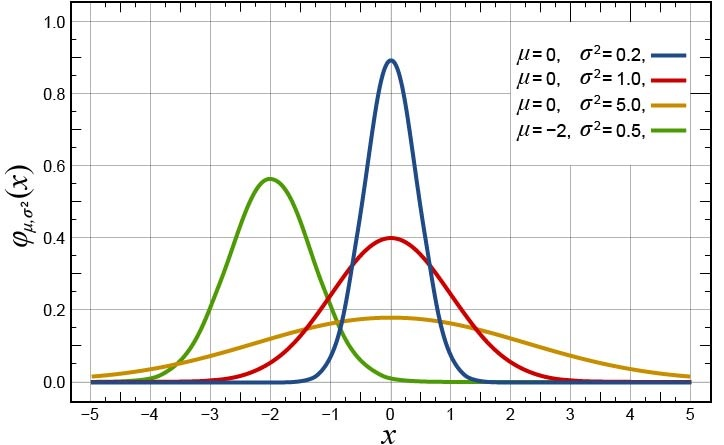
\includegraphics[width=0.8\textwidth]{Figures/Normal_Distribution_PDF.JPG}
\end{figure}

\end{frame}

\end{document}
